\chapter{Методология и окружение}\label{ch:chMethod}
Как упоминалось во Введении, для решения поставленной задачи - улучшения компилятора - необходимо определить неоптимальные места в коде, сгенерированным компилятором, которые при исполнении показывают недостаточную эффективность или вызывают задержку конвейера исполнения.

Во второй главе рассматривается методология поиска неоптимальностей в коде приложений и замера производительности. 

В разделе \ref{p1:platform} дается описание целевой платформы, под которую разрабатывались оптимизации.

В разделе  \ref{p1:tests} описаны два основных пакета приложений, на которых демонстрировались результаты разработанных методов.

В разделе \ref{p1:method} излагается методология получения результирующих цифр, основанная на многолетнем научном опыте.

В разделе \ref{p1:optop} приводятся основные методы изучений целевых приложений для последующей разработки компилятивных алгоритмов. Рассмотрены такие методы как профилирование, симуляция и обратная разработка.


\section{Целевая платформа}\label{p1:platform}

Для проведения исследований был выбран широко распространенный сервер компании Huawei - Kunpeng920. Он базируется на архитектуре ARM V8.2-A \cite{reid2016trustworthy,xia2021kunpeng}.  Основным конкурентом данного процессора на архитектуре ARM является Ampere Altra Server \cite{cha2021ampere}.  Исследуемая модель процессора создана по 7-нанометровой технологии и оснащена 64 ядрами с тактовой частотой 2.6 ГГц. Модель включает в себя  ряд аппаратных ускорителей, в том числе криптографии (MD5, HMAC, CMAC, AES, DES/3DES,  SHA1, SHA2) и  алгоритмов сжатия (GZIP, LZS, LZ4). 

Каждый чип состоит из двух вычислительных кристаллов (SCCL - Рисунок \ref{chip1})  и одного кристалл интерфейса (SICL - Рисунок \ref{chip2}). Кристалл интерфейса, соединенный через общую шину, содержит модуль ускорителя криптографии, интерфейсы ввода/вывода, PCIE и т.п. Каждый вычислительный кристалл содержит 8 кластеров центрального процессора (CCL). В свою очередь, кластер центрального процессора состоит из 4х вычислительных ядер, 4х блоков кэширования первого уровня (64К для данных и 64К для инструкций), 4х блоков кэшировния второго уровня и блока тэгов для кэша третьего уровня. Кэш третьего уровня располагается отдельно внутри вычислительного кристалла, присоединенный к общей шине, в нем также могут храниться данные из других вычислительных кристаллов. Каждое ядро представляет собой 4-х канальный суперскалярный модуль с возможностью изменения порядка исполнения (superscalar, out-of-order).

Интересной особенностью исследуемого процессора является широкая кэш-линия третьего уровня. Она составляет 128 байт, что в два раза превосходит общепринятое на рынке значение в 64 байта. 

\begin{figure}[htbp]
	\centering
	\includesvg[width = 300pt, inkscapelatex=false ]{SVG/wikichip1.drawio.svg}
	\caption{Схема целевого чипа}
	\label{chip1}
\end{figure}
\begin{figure}[htbp]
	\centering
	\includesvg[width = 300pt, inkscapelatex=false ]{SVG/SICL.drawio.svg}
	\caption{SICL модуль}
	\label{chip2}
\end{figure}

Поддерживаемые расширения:
\begin{itemize}
	\item  \textbf{NEON} - Векторное расширение ARMv8
	\item  \textbf{CRC32} - Расширение для быстрого подсчета чек-суммы CRC32
	\item  \textbf{Crypto} - Криптография
	\item  \textbf{FP16} - Числа с плавающей точкой половинной точности
	\item  \textbf{RAS} -  Надежность, доступность и удобство обслуживания. (Reliability, Availability, and Serviceability)
\end{itemize}

\section{Тесты производительности}\label{p1:tests}
\subsection{SpecCPU 2017}\label{p1:tests:spec}
В проведенном исследовании использовались два набора тестов: "SpecCPU 2017"\phantom{ } \cite{bucek2018spec} и CPUBench \cite{lu2023cpubench}. 

"SpecCPU 2017"\phantom{} - набор тестов для оценки производительности вычислительных систем. Существует два поднабора: целочисленный и набор тестов с плавающей арифметикой. Большая часть текущего исследования сосредоточена на улучшение производительности тестов с целочисленной арифметикой, однако некоторые общие подходы также применимы и к программам, использующим вычисления с плавающей точкой. Считается, что набор тестов SpecCPU является представителем современного рынка вычислений, поэтому многие компании при покупке вычислительных систем сравнивают производительность с использованием именно этого набора тестов \cite{bucek2018spec}.

Набор приложений, входящих в пакет "SpecCPU int 2017"\phantom{}:
\begin{itemize}
		\item  \textbf{perlbench}:  Интерпретатор языка Perl, из которого было удалено большинство особенностей, связанных с операционными системами. Включает в себя набор тестов, которые измеряют время выполнения различных операций в Perl \cite{siever1998perl}.
		\item  \textbf{gcc}: Известный компилятор языков С/C++/Fortran из коллекции компиляторов GNU \cite{gough2004introduction}. 
		\item  \textbf{mcf}: Моделирует задачу коммивояжера, где необходимо найти оптимальный маршрут для распространения товаров в различных городах, минимизируя расстояние и время пути \cite{lobel1999solving}.
		\item  \textbf{omnetpp}: OMNeT++ моделирует производительность  сети, используя алгоритмы и структуры данных для симуляции различных сценариев, таких как передача данных, маршрутизация и управление трафиком \cite{varga2019practical}.
		\item  \textbf{xalancbmk}: Моделирует преобразования XML-документов в HTML- или другие XML-документы с использованием языка XSLT (XSL Transformations) \cite{euzenat2002xml}.
		\item  \textbf{x264}: Свободная и открытая библиотека для кодирования видео, которая обеспечивает высококачественное и быстрое кодирование видео в формате H.264 (MPEG-4 AVC) \cite{merritt2006x264}.
		\item  \textbf{deepsjeng}: Искусственный интеллект игры в шахматы, имеет больше 2600 ELO  \cite{sandin2021ssdf}.
		\item  \textbf{leela}: Алгоритм игры в GO, включающий оценку позиции на основе метода Монте-Карло, выборочный поиск по дереву на основе верхних доверительных границ и оценку хода на основе рейтингов ELO \cite{choi2022does} .
		\item  \textbf{exchange2}: Программа, разработанная для генерации нестандартных и сложных судоку. Использовался на неофициальных соревнованиях, которые могли длиться несколько дней \cite{10.1145/1124708.1124709}. 
		\item  \textbf{xz}: Содержит компрессионный и декомпрессионный алгоритмы \cite{koranne2011compression}. 
\end{itemize}

Набор приложений, входящих в пакет "SpecCPU fp 2017"\phantom{}:
\begin{itemize}
	\item  \textbf{bwaves}:  Численное  моделирование взрывных волн. Первоначальная конфигурация задачи состоит из области высокого давления,  внутри которой находится небольшая область низкого давления. Сложная интерференционная  результирующая картина  решается при помощи уравнений Навье-Стокса \cite{auer1983intracranial}.
	\item  \textbf{cactuBSSN}: Моделирование черных дыр и гравитационных волн \cite{allen2007scientific}.
	\item  \textbf{namd}: Моделирование больших бимолекулярных систем. Почти все время выполнения тратится на расчет межатомных взаимодействий в небольшом наборе функций \cite{phillips2002namd}.
	\item  \textbf{parest}: Биомедицинская визуализация. Построение трехмерных моделей объектов из нескольких наблюдений на двумерной плоскости (например, МРТ, КТ) \cite{hoon2007fully}.
	\item  \textbf{povray}: Алгоритм трассировки лучей \cite{plachetka1998pov}.
	\item  \textbf{lbm}: Метод решеточных уравнений Больцмана для моделирования трехмерных моделей несжимаемых жидкостей.
	\item  \textbf{wrf}: Модель предсказания погоды, написанная на языке FORTRAN. Содержит огромное количество линейного кода \cite{skamarock2019description}. 
 	\item  \textbf{blender}: Рендер трех-мерных моделей \cite{brito2007blender}. 
 	\item  \textbf{cam4}: Модель циркуляции атмосферы \cite{neale2013mean}. 
 	\item  \textbf{imagick}: Производит последовательные манипуляции с двухмерной картинкой (повороты, отражения, размытие и т.д.) \cite{still2006definitive}. 
 	\item  \textbf{nab}: Приложение молекулярного моделирования, выполняющее интенсивные вычисления с плавающей запятой, которые обычно встречаются в области медико-биологических наук \cite{povcanic2009nab}. 
 	\item  \textbf{fotonik3d}: Вычисляет коэффициент передачи фотонного волновода, используя метод конечных разностей во временной области для уравнений Максвелла \cite{sullivan2013electromagnetic}.
 	\item  \textbf{roms}: Региональная система моделирования океана. Используется для исследования реакции океана на локальные изменения, такие как ветер или изменение температуры \cite{haidvogel2008ocean}. 
\end{itemize}



В наборе тестов SpecCPU существует два основных типа замера - speed и rate. В режиме speed разрешается использовать оптимизации с профилем, опции для каждого теста могут подбираться индивидуально. Однако в данной диссертации используется режим rate, в котором набор опций для всех тестов должен быть унифицирован и использование профиля запрещено. Запуск возможен как в режиме  одной копии - ресурсы машины доступны одному процессу полностью, так и  в режиме множественности копий, в котором процессам приходится делить общие ресурсы, такие как шину памяти или кэши. Стоит отметить, что ни в каком из наборов нельзя использовать прямо или косвенно информацию, специфичную для конкретных тестов. Так, например, в 2024 году более 2000 результатов  были помечены, как использующие информацию о тестах, а значит нечестные \cite{cliffFlagged}.

\subsection{CPUBench}\label{p1:tests:cpubench}

В 2023 году Китайский институт электроники и стандартизации выпустил новый набор тестов производительности для вычислительных систем \cite{lu2023cpubench}. В отличие от набора SpecCPU, интерфейс CPUBench разработан на языке python, а сам пакет имеет в себе программы, написанные на языке java. Авторами утверждается, что данный набор тестов является своеобразным расширением "SpecCPU 2017"\phantom{}, которое нацелено на лучшее покрытие мирового рынка (в том числе китайского). Было продемонстрировано на 14 различных платформах, что данный набор тестов сохраняет корреляцию производительности, показываемую пакетом SpecCPU.

Целочисленный набор состоит из следующих тестов:
\begin{itemize}
	\item  \textbf{x264, gcc, xz}: Схожие с пакетом "SpecCPU int 2017"\phantom{}, отличаются наборами входных данных и версиями приложений.
	\item  \textbf{gzip}: Архиватор, использующий алгоритм LZMA2 \cite{akoguz2016comparison}.
	\item  \textbf{tpcc}: Бенчмарк, который моделирует  деятельность розничного дистрибьютора с большим количеством складов и клиентов \cite{leutenegger1993modeling}.
	\item  \textbf{tpch}: База данных, состоящая из набора бизнес-ориентированных запросов и модификаций данных. Иллюстрируется система принятия решений \cite{barata2015overview}.
	\item  \textbf{kmeans}: Java тест, решающий задачу K-ближайших соседей.
	\item  \textbf{wordcount}: Java тест, подсчитывающий количество слов в больших файлах. 
	\item  \textbf{velvet}: Пакет алгоритмов, разработанный для сборки генома и выравнивания секвенирования коротких считываний \cite{zerbino2008velvet}. 
	\item  \textbf{openssl}: Криптографический инструментарий, реализующий различные алгоритмы шифрования \cite{rescorla2001introduction}.
	\item  \textbf{rapidjson}: Библиотека для парсинга Json -файлов \cite{keiser2023demand}
	\item  \textbf{python}: Интерпретатор языка Python \cite{python2021python}.
\end{itemize}
Набор тестов с плавающей точкой представлен следующим набором:
\begin{itemize}
	\item  \textbf{lightgbm}: Библиотека градиентного бустинга для машинного обучения \cite{ke2017lightgbm}.
	\item  \textbf{nektar}: Высокопроизводительный масштабируемый решатель для широкого спектра уравнений в частных производных \cite{cantwell2015nektar++}.
	\item  \textbf{phenglei}: Программная платформа вычислительной гидродинамики, разработанная Китайским центром исследований и разработок аэродинамики \cite{zhao2020design}.
	\item  \textbf{phyml}: Программа анализа белков и генов с помощью алгоритма максимального правдоподобия \cite{guindon2010new}.
	\item  \textbf{gromacs}: Пакет используется для моделирования различных биомолекул, имеющих большое количество межатомных связей \cite{van2005gromacs}.
	\item  \textbf{povray}: Алгоритм трассировки лучей \cite{plachetka1998pov}.
	\item  \textbf{openfoam}: Моделирование задач механики сплошных сред \cite{jasak2009openfoam}. 
	\item  \textbf{lammps}: Расчеты классической молекулярной динамики, применяется на суперкомпьютерах, имеет высокую степень парализации \cite{gowthaman2023review}.
	\item  \textbf{cube}: Гравитационная задача N-тел \cite{yu2018cube}.
	\item  \textbf{wrf}: Модель предсказания погоды, написанная на языке FORTRAN. Содержит огромное количество линейного кода \cite{skamarock2019description}. 	        
\end{itemize}

Можно заметить некоторую схожесть пакета "CPUBench int"\phantom{} с пакетом "SpecCPU int"\phantom{}. Так, вместо интерпретатора языка perl представлен интерпретатор более современного языка python, добавлен дополнительный алгоритм компрессии/декомпрессии, парсинг XML документов заменен на парсер JSON файлов. А вот алгоритмов искусственного интеллекта здесь не наблюдается, зато присутствую базы данных MySQL и криптографический инструмент openssl.

Что касается тестов с плавающей точкой, большинство представленных программ в SpecCPU можно разделить на 2 категории: работа с графическими объектами и научные вычисления, в то время как в пакете CPUBench из графических приложений можно увидеть только алгоритм трассировки лучей, однако CPUBench содержит в себе библиотеку градиентного бустинга lightgbm, активно применяющуюся в машинном обучении. 

\section{Методология измерения}\label{p1:method}
В данной диссертаций используется измерения типа  "SpecCPU rate"\phantom{} и ее аналог typcal в CPUBench. В данной методологии предусмотрены следующие шаги:
\begin{enumerate} 
		\item Измерение времени выполнения каждого теста, запущенного в $NUM\_COPIES$ копий, в некоторое количество итераций ($N$)
		\item Если было запущено больше одной копии, то временем исполнения теста считается самое большое время среди всех копий.
		\item Для каждого теста выбирается медианное время среди проделанных итераций. 
		\item Обратное медианное время каждого теста умножается на референсное время ($REF\_TIME$), полученное на фиксированной машине. Например, для "SpecCPU 2017"\phantom{} это  Sun Fire V490 with 2100 MHz UltraSPARC-IV+.
		\item Считается среднее геометрическое по всем тестам. Использование среднего геометрического обосновывается свойством сохранения отношения.
		\item Полученное число умножается на количество копий.
\end{enumerate}
Если всего в сете $M$ тестов, то кратко можно записать формулу расчета производительности следующим образом:
\begin{equation}
RATE =\left(\prod _{i=1}^{M}\dfrac{REF\_TIME_i}{MEDIAN(TIME_{i1}, TIME_{i2}, ... , TIME_{iN})}\right)^{\frac {1}{M}} 
\end{equation}

Также важной частью считается настройка окружающей системы, направленная на уменьшение флуктуаций времени исполнения тестов и лучшей утилизации тестовой системы.
Эта тема не является прямой темой данного исследования, а лишь косвенного затрагивает ее, но тем не менее весьма важна,поэтому ниже предлагается ознакомится с проблемами, которыми пришлось столкнуться во  время проведения замеров для алгоритмов, реализованных в данной диссертации.  

\begin{itemize}
	\item  \textbf{Троттлинг}. Технология изменения частоты процессора при превышении критических температур. Часто возникает при нарушении системы охлаждения или неправильной эксплуатации. Проявляется в виде увеличения времени исполнения теста с каждой следующей итерацией \cite{zhang2009hardware}.
		\begin{figure}[ht]
		\centerfloat{
			\includegraphics[scale=1]{PNG/ddr1}
		}
		\caption{Схема подсистемы памяти целевой платформы}\label{fig:ddrsvg1}
	\end{figure}
	\item  \textbf{Неполная утилизация ресурсов системы}. Целевая платформа имеет восемь каналов DRAM, с возможностью подключения до двух плашек на каждый канал (Рисунок \ref{fig:ddrsvg1}). В случае, если какой-то канал остался незадействованным (Например, вставлены подряд, а не через одну) то будет наблюдаться картина, как на рисунке \ref{fig:lack_of_memmory}. Можно видеть, что неиспользуемые порты приводят к тому, что вычислительным ядрам приходится обращаться за ресурсами памяти в соседние блоки, что значительно замедляет исполнение.

	
	\begin{figure}[ht]
		\centerfloat{
			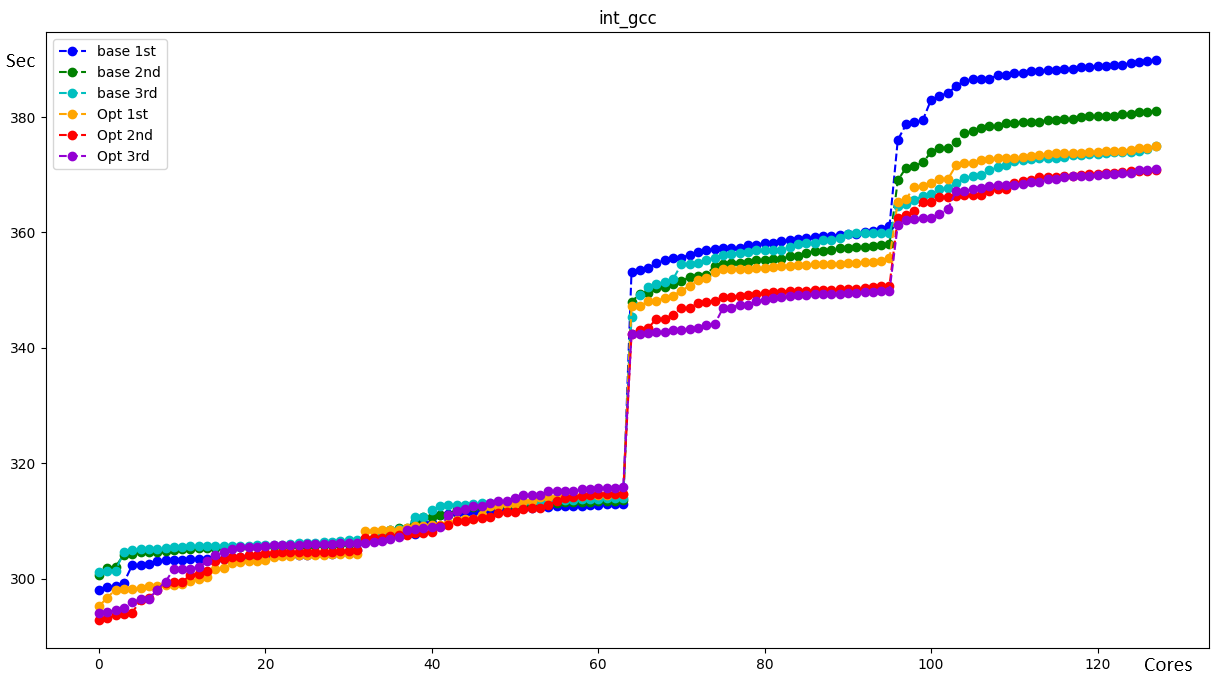
\includegraphics[scale=0.5]{PNG/lack_of_memmory}
		}
		\caption{Зависимость времени исполнения приложения от номера ядра при неправильном подключении плашек оперативной памяти}\label{fig:lack_of_memmory}
	\end{figure}
	\item \textbf{Рандомизация размещения адресного пространства (ASLR)}. Технология, изначально разрабатываемая для защиты процессов от различного рода атак с использованием  переполнения буфера. При этом  адреса расположения исполняемого файла рандомизируются для усложнения предсказания положения объекта в памяти и получения доступа из сторонних процессов \cite{gras2017aslr}. Однако, в случае аккуратных измерений производительности системы эта технология может приводить к случайному наложению младших частей адресов и, соответственно, попаданию в одну и ту же кэш линию. На рисунке \ref{fig:peaks}  можно видеть как на случайном ядре время исполнения отдельной копии увеличивается больше, чем в 2 раза.
	\item \textbf{Частота обновления оперативной памяти} - Оперативная память, являясь энергозависимой памятью, требует постоянного обновления значений в ячейках. Частота обновления этих ячеек регулируется в BIOS. С одной стороны, большая частота обновления уменьшает количество ошибок и связанных с ними задержек, однако с другой стороны, обновление памяти это по своей сути дополнительная загрузка данных, что в высоко нагруженной системе может создавать дополнительные задержки. Поэтому этот параметр приходится подбирать эмпирическим путем, и он оказывает существенное влияние на итоговую производительность системы.
	
	\begin{figure}[ht]
		\centerfloat{
			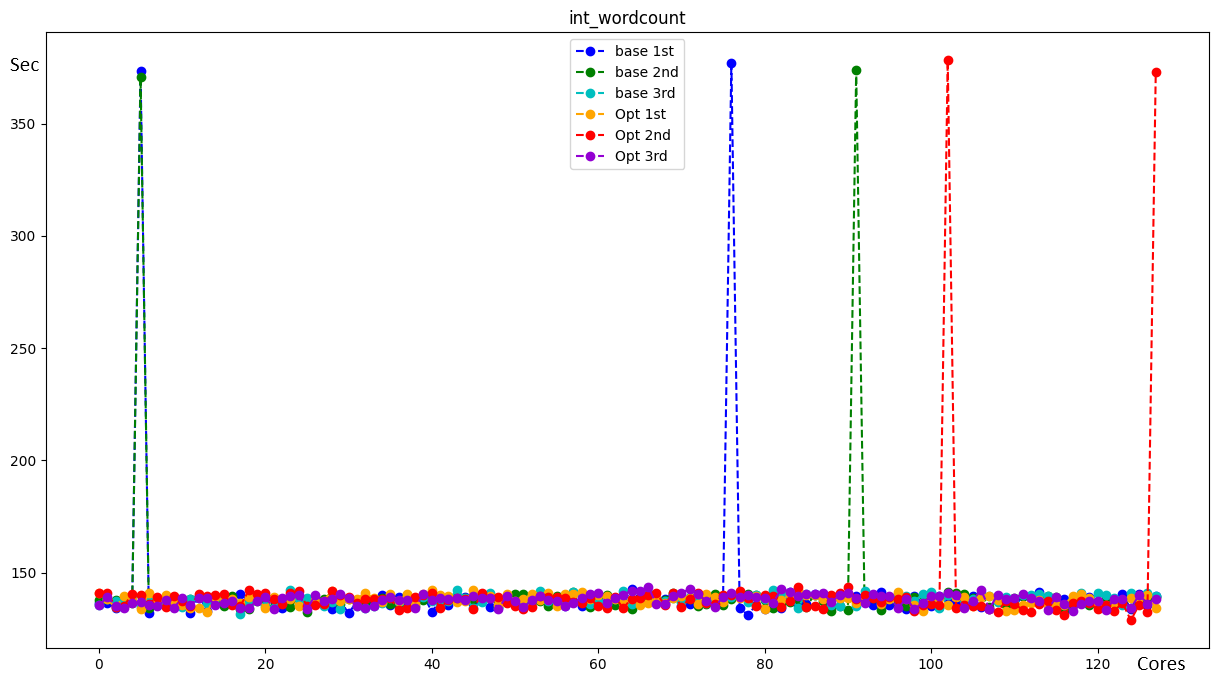
\includegraphics[scale=0.5]{PNG/peaks}
		}
		\caption{Зависимость времени исполнения приложения от номера ядра при замере c включенной ASLR}\label{fig:peaks}
	\end{figure}
	\item \textbf{Занятость ресурсов внешними программами}. Достаточно очевидный факт: если необходимо измерить производительность системы, то ваш бенчамрк должен быть единственным, исполняемым на этой системе.  Однако, организовать тест в изоляции достаточно сложно, так как операционная система время от времени может запускать демонов, планировщик и прочее,  методы борьбы с этим индивидуальны и не будут указаны здесь, однако, покажем, как пронаблюдать этот эффект. Если мы производим высокоинтенсивной замер, утилизирующий все ядра и большинство остальных ресурсов системы, а затем отсортируем время выполнения тестов на разных ядрах, то можем получить картину, как на рисунке \ref{fig:tails}. Эти "хвосты"\  чаще всего означают, что система была занята другими  приложениями, а не  тестом.
\end{itemize}


\begin{figure}[ht]
	\centerfloat{
		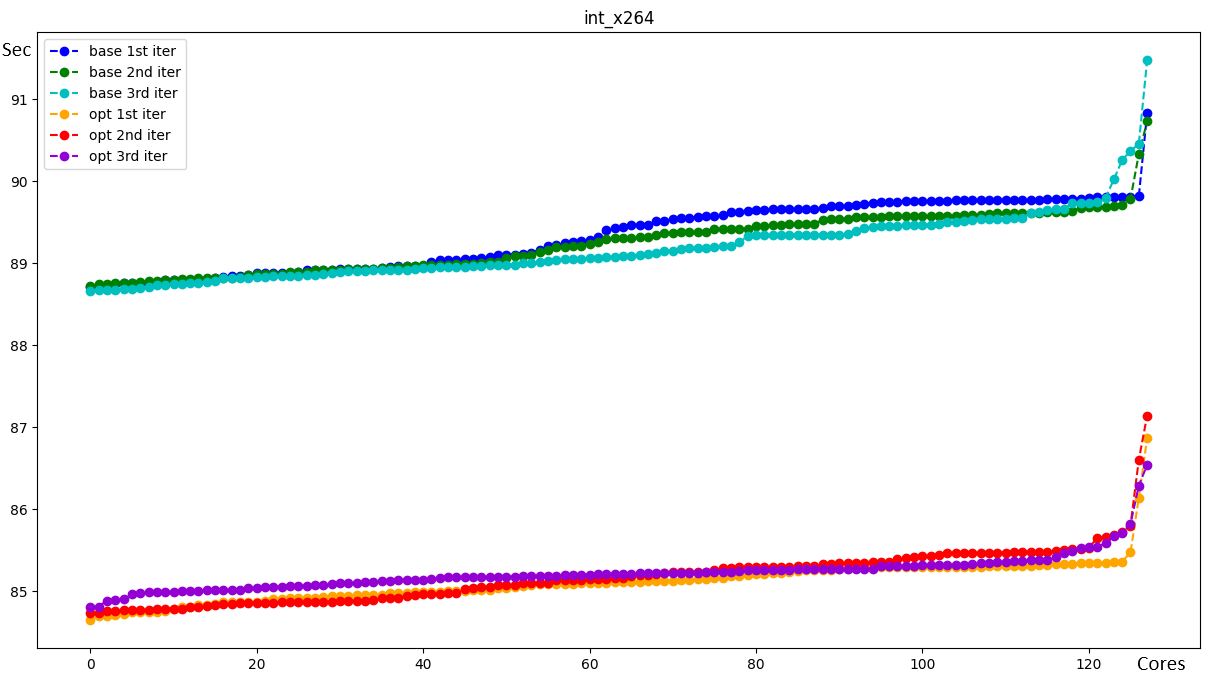
\includegraphics[scale=0.5]{PNG/tails}
	}
	\caption{Зависимость времени исполнения приложения от номера ядра при замере на загруженной системе}\label{fig:tails}
\end{figure}



Приведенные проблемы нельзя решить после замера каким-либо "обрезанием хвостов"\  или "удалением пиков"\  из выборки. Методология такого не позволяет. Если бы подобные манипуляции были возможны, то это позволило бы вендорам манипулировать данными, ведь тогда пришлось бы вводить какие-либо правила, когда и как можно корректировать данные замеров, что привело бы к махинациям ради получения более высоких цифр производительности.

\section {Выявление возможностей для оптимизации}\label{p1:optop}
Данное исследование подразумевает выявление оптимизационных возможностей тестовых приложений для последующей разработки оптимизаций. К сожалению, очень сложно предоставить определенный алгоритм поиска оптимизационных возможностей, так как разные программы оказывают нагрузку разного типа на систему, подход к каждому случаю практически индивидуален, и должен учитывать аппаратные возможности, архитектуру команд и структуру исходной программы. Однако существуют достаточно понятные методологии поиска горячих (высоконагруженных) участков. Рассмотрим методы, которые использовались в данной диссертационной работе.

\subsection {Профилирование}\label{p1:optop:profile}
\textbf{Профилирование программы}  - это методика динамического анализа программы, которая способна измерить количество вызовов функций, загруженность памяти, использование определенных инструкций,  временную сложность программы.

Программы профилирования приложений в зависимости от способа сбора информации можно глобально разделить на три типа:

Первый тип профилирующих программ базируется на событиях, которые происходят внутри программы. Для этого в код самого приложения или в код подгружаемых библиотек  вставляются дополнительные обработчики на этапе компиляции или линковки приложения. В процессе исполнения программа непосредственно перед заранее определенным программным событием (вызов функции, аллокация памяти, создание объекта и пр.) вызывается встроенным метод-обработчик, который собирает и агрегирует полезную профильную информацию. Классическим примером такого профилировщика является \textbf{gprof} \cite{graham2004gprof}. При таком способе внутрипрограмные события собирается с высокой точностью, однако постоянный запуск обработчиков может искажать перфомансную картину приложения (перебивать данные в кэшах и  влиять на логику предсказателей). Огромным минусом данной модели является необходимость перекомпиляции программы.

Другой подход - интерпретирующие профилировщики, по своей сути являющиеся бинарными трансляторами/интерпретаторами с возможностью выставления любых программных счетчиков непосредственно в код исполняемой программы во время исполнения \cite{reinders2005vtune, nethercote2007valgrind}. Являются мощнейшими инструментами профилирования, однако оказывают сильное влияние на время исполнение программы, замедляя ее в десятки или даже сотни раз. Тем не менее такой подход не требует перекомпиляции самого приложения и обладает высокой точностью сбора внутрипрограммных событий.

Третий подход и один из основных методов выявления оптимизационных возможностей в рамках данной диссертационной работы -  сэмплирующий профилировщик \textbf{perf} \cite{de2010new}. Он способен проверять стек вызовов программы через регулярные промежутки времени, благодаря интерфейсу прерываний операционной системы. Профили, собранные таким образом, обычно менее точны и не очень конкретны (могут пропускать вызовы функций), однако позволяют измеряемой программе работать практически на полной скорости. Относительная точность достигается путем агрегации большого количества данных. Такой тип профилирования наиболее удобен для больших приложений, используемых пользователями.


Важной особенностью сборки профильной информации является поддержка аппаратных счетчиков в архитектуре ARM64, реализованная в виде PMU (Performance Monitoring Unit). PMU это специализированный блок процессора, предназначенный для отслеживания различных событий, которые происходят на уровне микроархитектуры \cite{hansen2020examining}. PMU может быть управляем через специальные инструкции, такие как MCR (Move to Coprocessor from Register) и MRC (Move to Register from Coprocessor), позволяющие записывать и считывать данные из блока-монитора. Для контроля этого устройства существует 32 программируемых счетчика, которые могут быть настроены для отслеживания различных событий. Каждый счетчик может быть настроен для отслеживания конкретного события. В качестве примера событий, которые могут быть собраны благодаря PMU, можно привести:
\begin{itemize}
	\item Промахи в L1/L2/L3 кэш.
	\item Задержки в очереди на исполнение.
	\item Задержки, связанные с "голодом"\phantom{} исполняющих устройств (нет доступных для исполнения инструкций).
	\item Ошибки предсказания переходов.
	\item Задержки фронт-енда аппаратуры.
	\item Количество векторных инструкций.
	\item Количество инструкций с плавающей точкой. (метрика недоступна на исследуемой машине)
\end{itemize}


Такой метод позволяет очень сильно сузить круг поиска возможных оптимизаций. Так, например, в тестах xz и gzip наблюдалось значительное количество задержек в память, что в последующем послужило мотивацией к разработке дополнительных алгоритмов программной предподкачки данных. В тестах openssl, tpcc, tpch, python наблюдалось высокое количество задержек, связанных с фронт-ендом аппаратуры, частые ошибки предсказания переходов. В последующем этот анализ дал толчок к разработке оптимизации свертки условных переходов. Малое количество векторизованного кода в x264 привело к улучшению алгоритма векторизации.


\subsection {Симуляция}\label{p1:optop:sim}

Иногда общих соображений из главы \ref{p1:optop:profile} недостаточно для определения причин замедления программы. В таких случаях можно произвести исследование на потактововом симуляторе данной машины или близкой к ней по конфигурации и временным параметрам, при отсутствии точной модели. В качестве примера приведем пример анализа из оригинальной работы, посвященной оптимизации инструкций широкого доступа в память \cite{chernonog2024widemem}, позволившее реализовать оптимизацию \ref{ch2:split_ldp_stp}.

В качестве потактовой модели был использован симулятор GEM5, содержащий детальную модель микроархитектуры процессора Alpha 21264 \cite{lowe2020gem5,qiu2023performance}. Конфигурация симулируемой системы приведена в таблице \ref{tab:setupsim}. Важно подчеркнуть, что моделирование осуществляется в режиме эмуляции системных вызовов (system emulation), в котором отсутствует исполнение кода ядра операционной системы. 

\begin{table} [htbp]
	
	\raggedright
	\begin{threeparttable}% выравнивание подписи по границам таблицы
		\caption{Настройка симулируемой модели}\label{tab:setupsim}%
		\begin{tabular}{ | m{5cm} | m{8cm} l|}
			\hline
			\hline
			\centering Архитектура			 & \centering  ARMv8.2-A & \\
			\hline
			\centering Модель процессора			 & \centering ArmO3CPU  & \\
			\hline
			\centering Кэш-память L1			 & \centering 64 кБ кэш данных, 64 кБ кэш инструкций  & \\
			\hline
			\centering Кэш-память L2			 & \centering 512 кБ, общий  & \\
			\hline
			\centering Ширина этапов конвейера			 & \centering 4 для всех этапов  & \\
			\hline
			\centering Количество LSU блоков & \centering 2   & \\
			\hline
			\centering Оперативная память 	& \centering  DDR4 2400 МГц 512 МБ  & \\
			\hline
			\hline
		\end{tabular}
	\end{threeparttable}
\end{table}


\begin{figure}[ht]
	\centerfloat{
		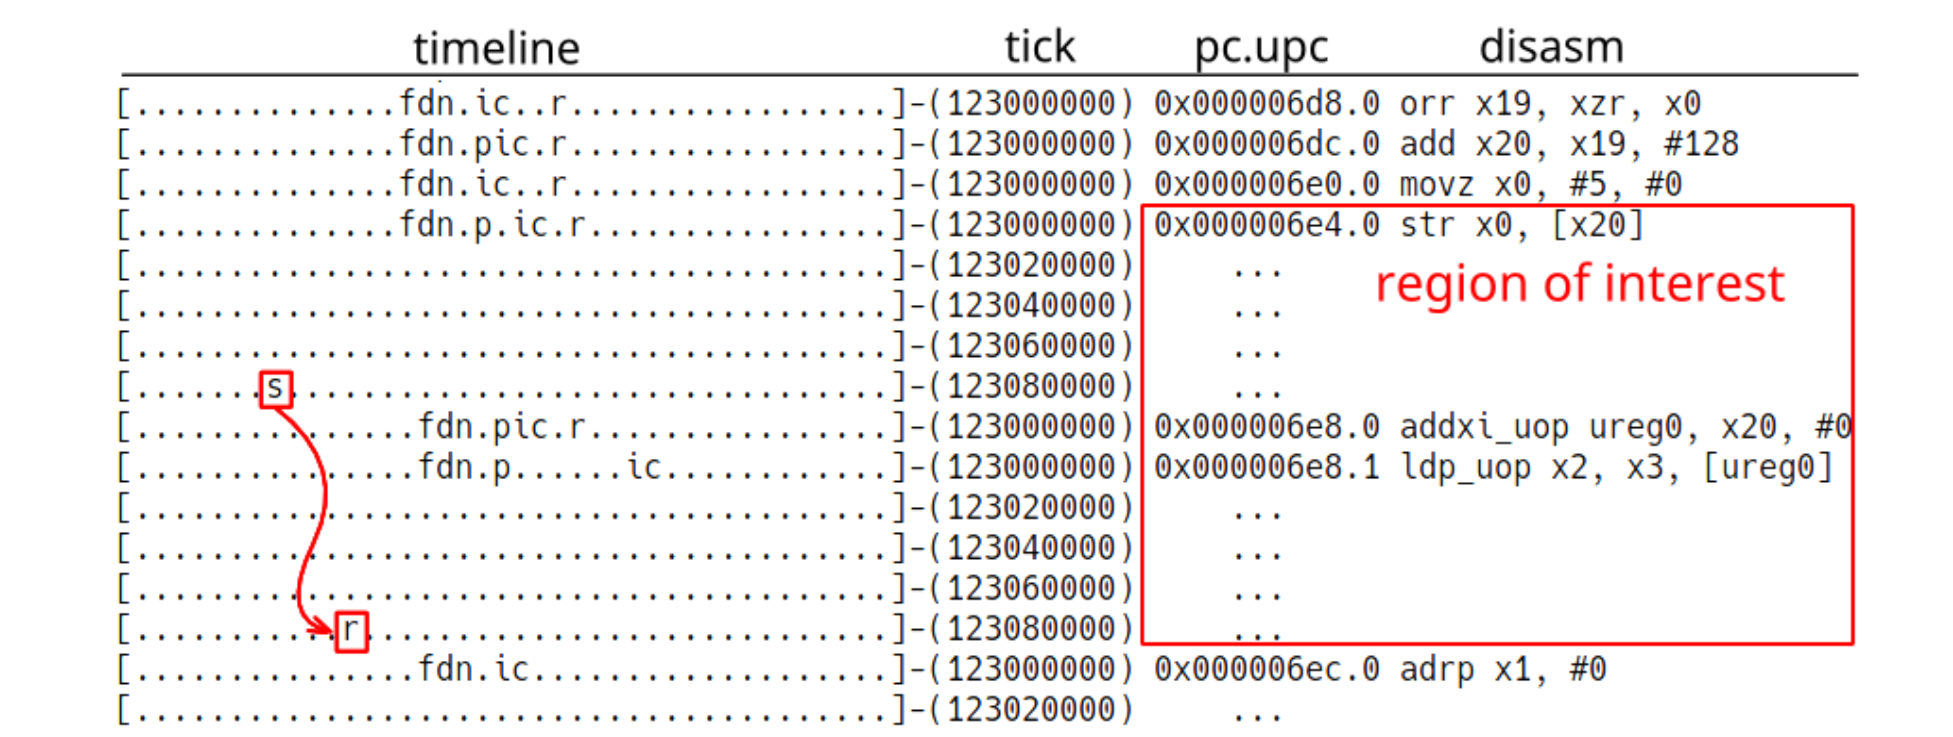
\includegraphics[scale=0.35]{PNG/simstep1}
	}
	\caption{Моделирование исполнения широкой инструкции чтения после записи}\label{fig:simstep1}
\end{figure}
\begin{figure}[ht]
	\centerfloat{
		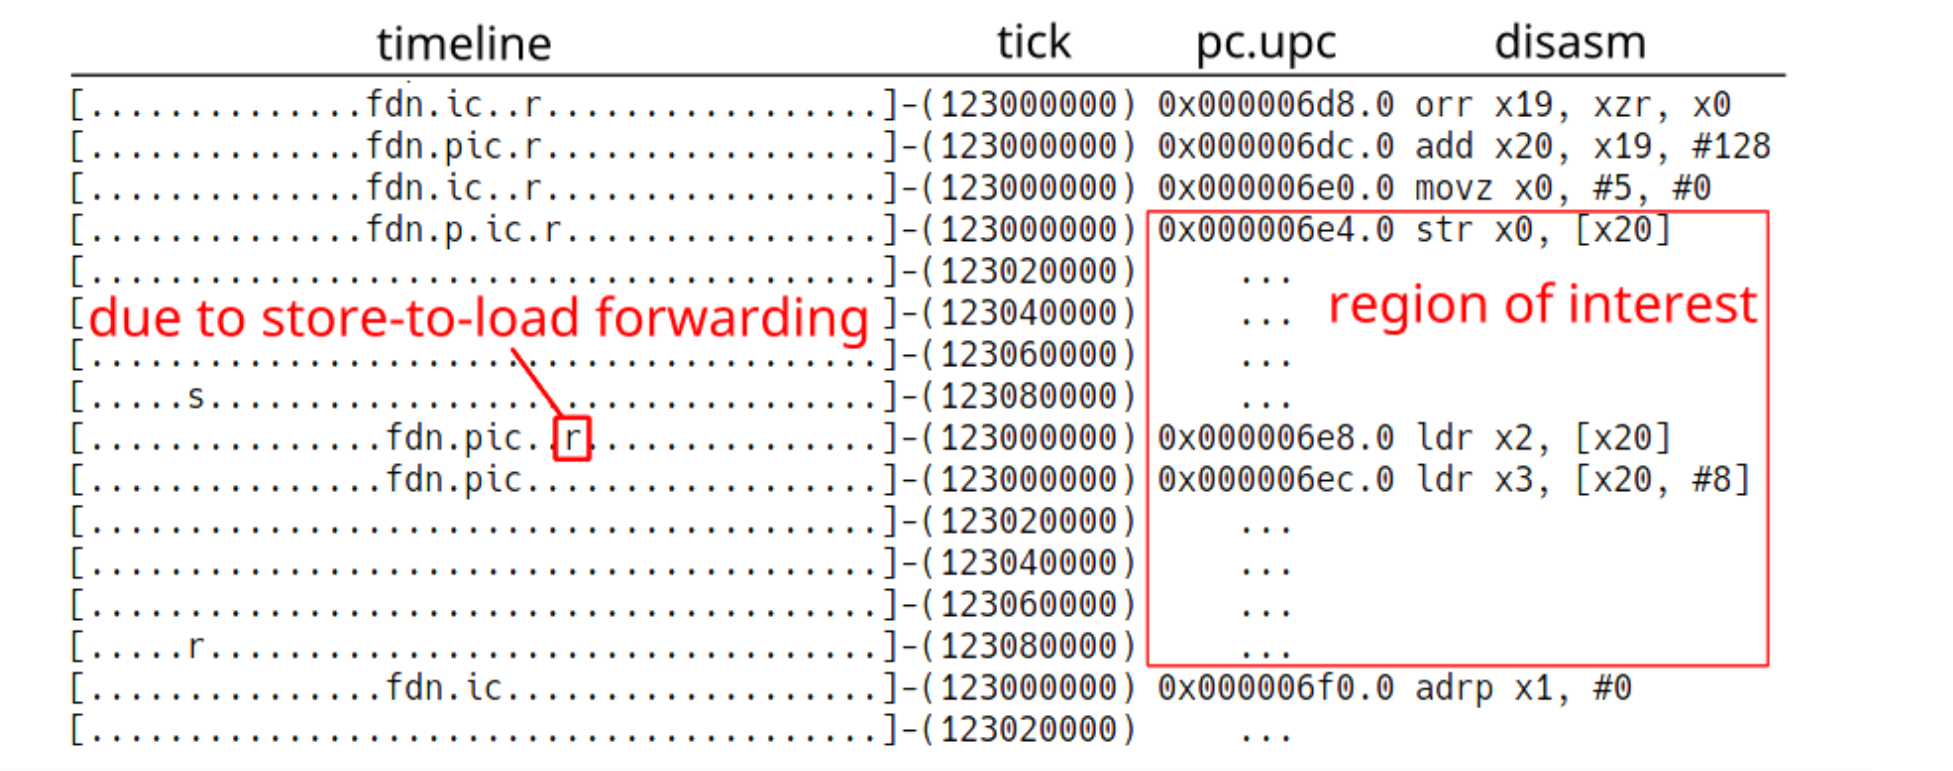
\includegraphics[scale=0.35]{PNG/simstep2}
	}
	\caption{Моделирование исполнения двух инструкций, полученных в результате разбиения широкой инструкции чтения памяти}\label{fig:simstep2}
\end{figure}
\begin{figure}[ht]
	\centerfloat{
		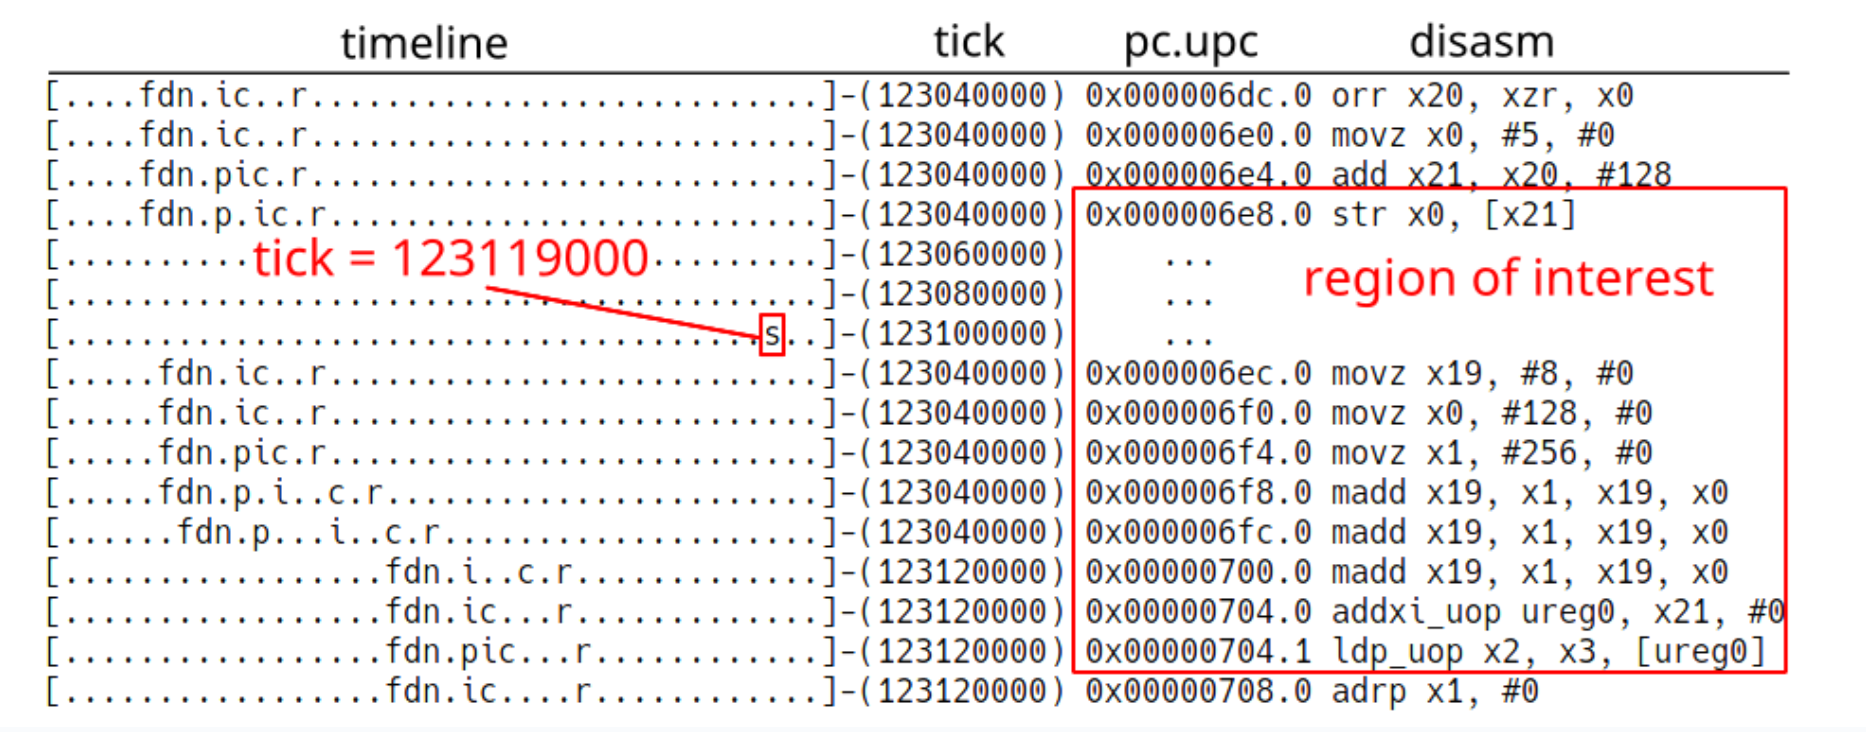
\includegraphics[scale=0.35]{PNG/simstep3}
	}
	\caption{Моделирование исполнения арифметических операций перед широкой инструкцией доступа в память}\label{fig:simstep3}
\end{figure}
\begin{figure}[ht]
	\centerfloat{
		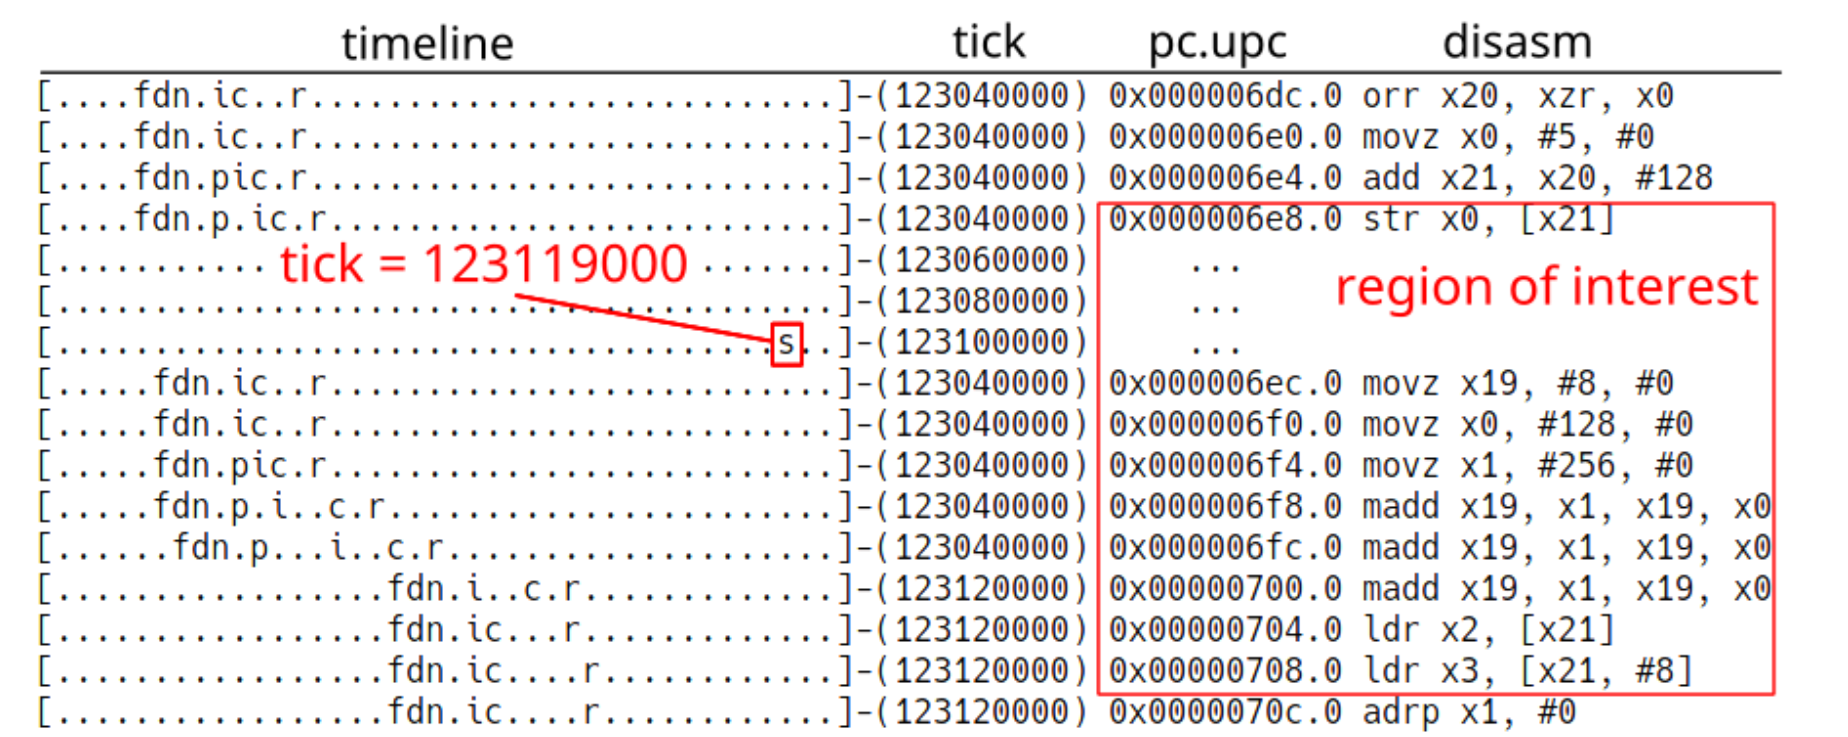
\includegraphics[scale=0.35]{PNG/simstep4}
	}
	\caption{Моделирование исполнения арифметических операций перед двумя инструкциями, полученными в результате разбиения широкой инструкции чтения}\label{fig:simstep4}
\end{figure}

На рисунке \ref{fig:simstep1} приводится код, содержащий инструкции записи (STR) и  широкого чтения (LDP) с одинаковым базовым регистром. 
В левой части рисунка располагается временная шкала. Каждая точка соответствует одному циклу центрального процессора, там же указаны стадии конвейера:
\begin{enumerate}
\item f - fetch - чтение инструкции из ячейки памяти 
\item d - decode - разбор инструкции и ее аргументов
\item n - rename - переименование регистров (маппинг на физические)
\item p - dispatch - отправка инструкции в бек-енд (back-end) процессора
\item i - issue - назначение конкретного вычислительного устройства
\item c - complete - окончание исполнения
\item r - retire - возвращение результата операции пользователю
\item s - store-complete - завершение операции записи в память 
\end{enumerate}

В рассматриваемом сценарии процессором выполняется чтение, реализованное через инструкцию LDP, 16 байт данных, но перед чтением с помощью инструкции STR обновляются 8 байт в том же диапазоне памяти. Возникающий конфликт называется зависимостью "чтение после записи". Видно, что разбитая на микрооперации инструкция LDP переходит на этап r (retire) только спустя 4 такта после завершения записи в память.





На рисунке \ref{fig:simstep2} проиллюстрирована работа  аппаратного механизма разрешения зависимостей при спекулятивном выполнении операций доступа в память. Видно, что задержки не происходит.

Между рассматриваемыми инструкциями чтения и записи процессором могут выполняться прочие операции, и к моменту начала исполнения операции чтения запись в память полностью завершится. Моделирование такой ситуации для двух ранее рассмотренных случаев продемонстрировано на рисунках \ref{fig:simstep3} и \ref{fig:simstep4}. В обоих случаях на чтение пары значений тратится одинаковое время, так как в очереди на запись уже нет данных, которые можно взять для первой инструкции чтения. Следовательно, разделение инструкции широкого доступа не всегда целесообразно и требует анализа. В общем случае максимальное число инструкций между двумя конфликтующими операциями доступа в память, которое далее будем называть дистанцией, зависит от конфигурации конкретного процессора и времени выполнения инструкций различного типа, поэтому предлагается определять это значение эмпирическим путем.

\subsection{Обратная разработка}\label{p1:optop:reverse}

Чаще всего под обратной разработкой понимают исследование некоторого готового продукта с целью изучения его свойств. Конечно же в проделанной работе тоже имелся такой этап. Для целевого оптимизатора конкурентами являются такие компиляторы как LLVM Clang \cite{lattner2008llvm} и intel DPC++ \cite{castano2022evaluation}. Обратная разработка позволяет провести быстрый визуальный анализ сгенерированного кода и, что самое важное,  модифицировать его без необходимости перекомпиляции. Среди существующих популярных инструментов дизассемблера (IDA, Radare2, Ghidra и др. \cite{ferguson2008reverse, mester2023malware, jiang2022comprehensive}) был выбран radare2. Его преимуществами являются четкое описание установки на своей странице Github, наличие обширной документации и поддержки сообщества на своей странице Wikipedia и своей официальной электронной книге. Пример выводимой информации приложением radare2 можно увидеть на рисунке \ref{radare2}.

\begin{figure}[ht]
	\centerfloat{
		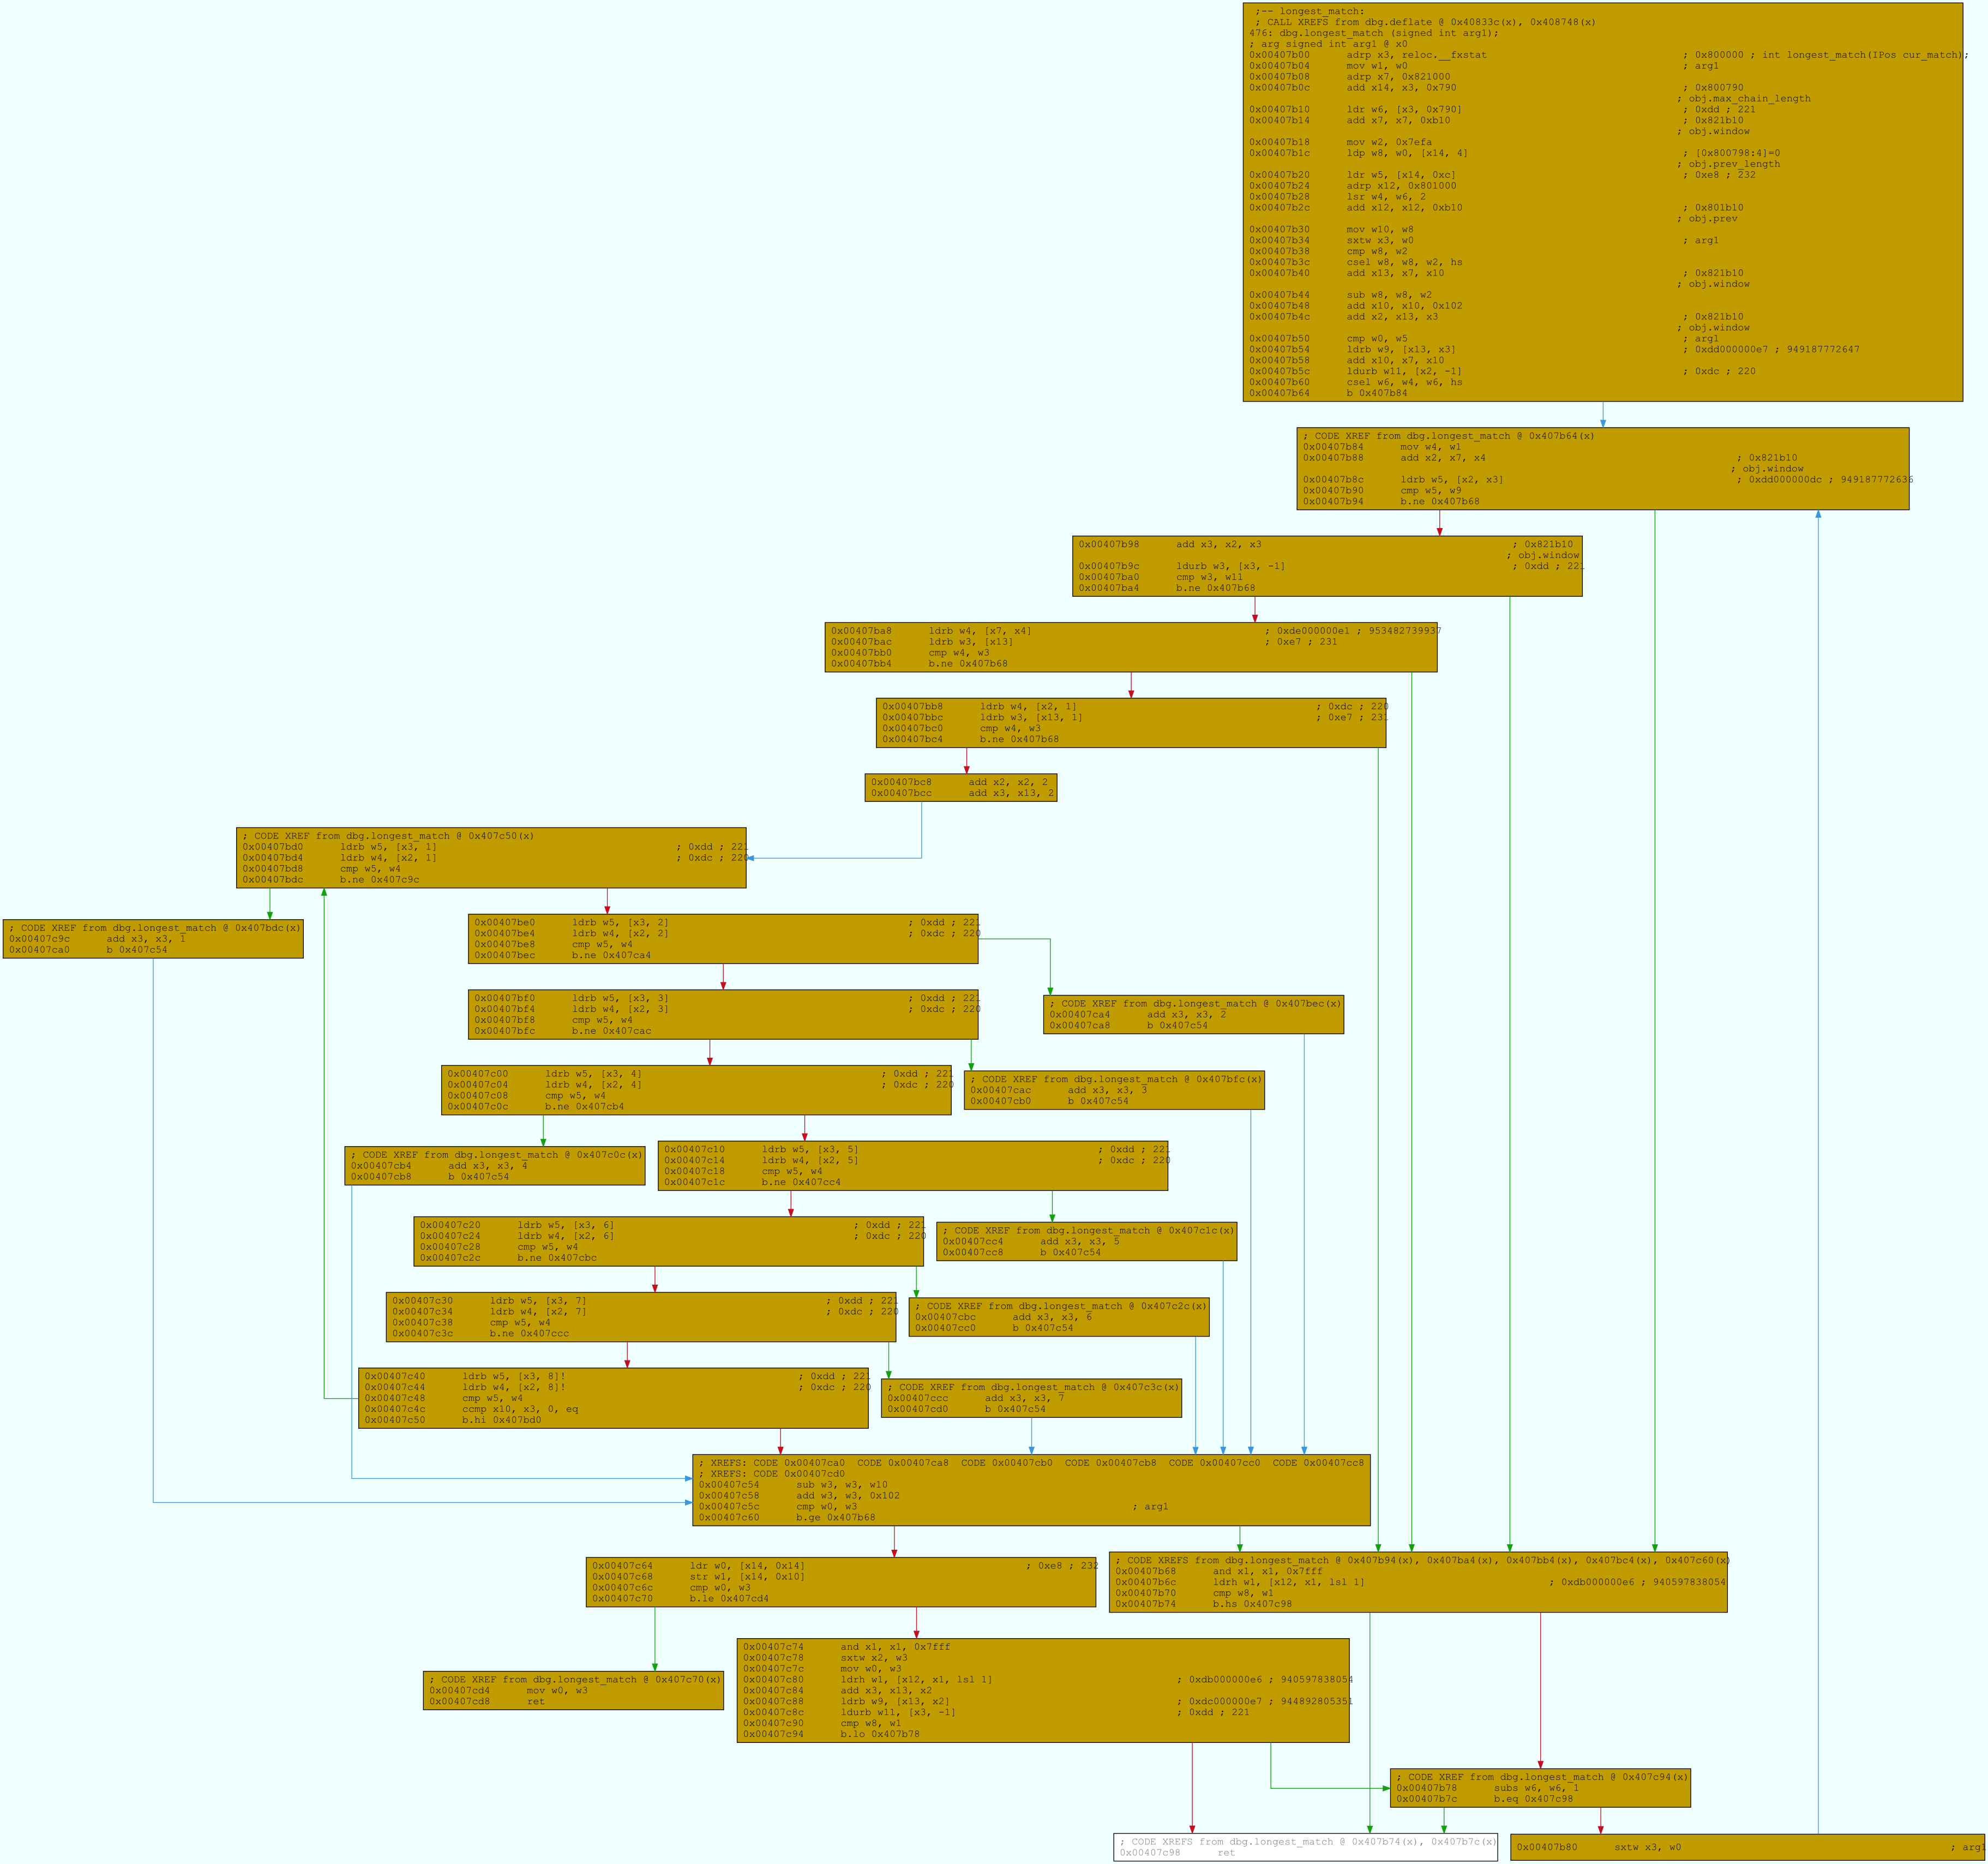
\includegraphics[scale=0.18]{PNG/gzip_longest_match}
	}
	\caption{Базовые блоки горячего участка кода приложения gzip, полученные с помощью radare2}\label{radare2}
\end{figure}

\section{Выводы по главе}

Во второй главе приводится описание целевой архитектуры,  методы исследования приложений и замера цифр производительности. 

Рассмотрены проблемы, связанные с процессом измерения цифр производительности, описаны их архитектурные причины.

На примерах исследуемых приложений показано использование программного обеспечения для анализа тестов на целевой архитектуре.



